%auto-ignore

\section{관련 연구}
일반적인 언어 표현을 사전학습하는 시도는 오랜 역사를 갖고 있으며, 본 절에서는 가장 널리 쓰여 온 접근들을 짧게 살펴본다.


\subsection{비지도 피처 기반 접근}
폭넓게 적용 가능한 단어 표현(word representation)을 배우는 일은 수십 년 동안 활발한 연구 주제였으며, 비-신경망(non-neural) 방식~\cite{brown-etal:1992:_class, ando-zhang:2005, blitzer-mcdonald-pereira:2006:_domain}과 신경망(neural) 방식~\cite{mikolov-etal:2013, pennington-socher-manning:2014:_glove}을 모두 포함한다. 사전학습된 단어 임베딩(word embedding)은 현대 NLP 시스템의 핵심 구성요소이며, 처음부터 학습된 임베딩에 비해 큰 폭의 향상을 제공한다~\cite{turian-ratinov-bengio:2010:_word_repres}. 단어 임베딩 벡터를 사전학습하는 데에는 좌→우 언어모델링 목적함수가 사용되었고~\cite{minh09}, 좌·우 맥락에서 올바른 단어와 잘못된 단어를 구분하는 목적함수도 사용되었다~\cite{mikolov-etal:2013}.

이러한 접근은 문장 임베딩(sentence embedding)~\cite{kiros-etal:2015:_skip, logeswaran2018an}이나 단락 임베딩(paragraph embedding)~\cite{le-mikolov:2014:_distr} 같은 더 굵은 단위로도 일반화되었다. 문장 표현을 학습하기 위해 기존 연구는 후보 다음 문장의 순위를 매기는 목적함수~\cite{DBLP:journals/corr/JerniteBS17, logeswaran2018an}, 이전 문장의 표현이 주어졌을 때 다음 문장의 단어를 좌→우로 생성하는 목적함수~\cite{kiros-etal:2015:_skip}, 또는 잡음제거 오토인코더(denoising auto-encoder)에서 유도된 목적함수~\cite{hill16}를 사용해 왔다.

%
\begin{figure*}[t!]
%\small
\begin{center}
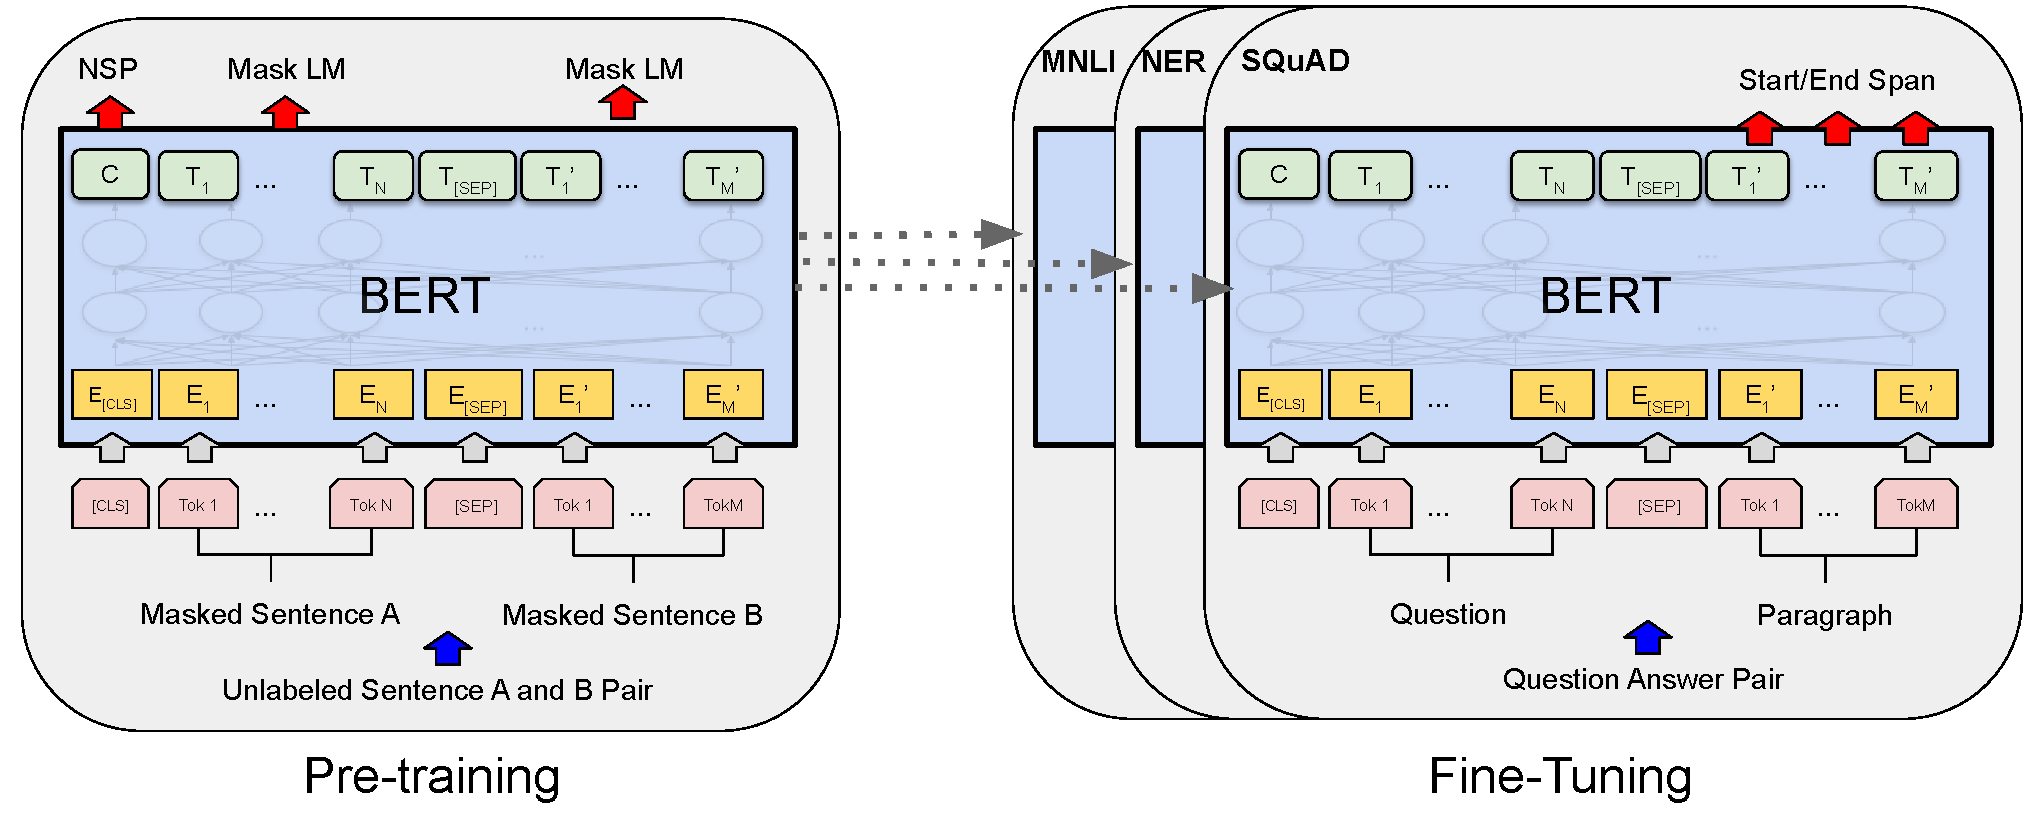
\includegraphics[width=1\textwidth]{BERT_Overall.pdf}
\end{center}
\caption{BERT의 전체 사전학습 및 파인튜닝 절차. 출력 층을 제외하면 사전학습과 파인튜닝에 동일한 아키텍처가 사용된다. 동일한 사전학습 모델 파라미터로 서로 다른 다운스트림 과제용 모델을 초기화하고, 파인튜닝 동안에는 모든 파라미터가 갱신된다. {\tt [CLS]}는 모든 입력 예시의 앞에 추가되는 특수 기호이며, {\tt [SEP]}는 특수 분리 토큰이다(예: 질문/답변 분리).}
\label{fig:bert_overall}
\end{figure*}
%



ELMo와 그 선행 연구~\cite{peters-etal:2017:_semi, peters-etal:2018:_deep}는 전통적인 단어 임베딩 연구를 또 다른 차원으로 일반화했다. 이들은 좌→우와 우→좌 언어모델로부터 \emph{맥락 민감(context-sensitive)} 피처를 추출한다. 각 토큰의 맥락 표현은 좌→우와 우→좌 표현의 결합이다. 맥락적 단어 임베딩을 기존의 과제별 아키텍처와 결합함으로써, ELMo는 질의응답~\cite{rajpurkar-etal:2016:_squad}, 감성 분석(sentiment analysis)~\cite{socher-etal:2013:_recur}, 개체명 인식~\cite{tjong-de:2003}을 포함한 여러 주요 NLP 벤치마크(benchmark)의 최첨단을 갱신했다~\cite{peters-etal:2018:_deep}.
\citet{melamud2016context2vec}은 LSTM을 이용해 좌·우 맥락 모두에서 단일 단어를 예측하는 과제를 통해 맥락 표현을 학습할 것을 제안했다. ELMo와 마찬가지로, 이 모델도 피처 기반이며 깊게 양방향이지는 않다.
\citet{fedus2018maskgan}은 cloze 과제를 텍스트 생성 모델의 견고성 향상에 활용할 수 있음을 보였다.




\subsection{비지도 파인튜닝 접근}

피처 기반 접근과 마찬가지로, 이 방향의 초기 연구도 비라벨 텍스트로부터 단어 임베딩 파라미터만 사전학습했다~\cite{collobert-weston:2008}.

더 최근에는, 맥락 토큰 표현을 만들어 내는 문장 또는 문서 인코더가 비라벨 텍스트로부터 사전학습된 뒤, 지도 학습 다운스트림 과제에 파인튜닝되어 왔다~\cite{dai-le:2015:_semi, howard-ruder:2018, radford-etal:2018}. 이 접근의 장점은 처음부터 학습해야 하는 파라미터가 적다는 점이다. 적어도 부분적으로 이 장점에 힘입어, OpenAI GPT~\cite{radford-etal:2018}는 GLUE 벤치마크~\cite{wang-etal:2018:_glue}의 많은 문장 수준 과제에서 이전의 최첨단을 달성했다. 그러한 모델의 사전학습에는 좌→우 언어모델링과 오토인코더 목적함수가 사용되어 왔다~\cite{howard-ruder:2018, radford-etal:2018,dai-le:2015:_semi}.




\subsection{지도 데이터로부터의 전이 학습}

자연어 추론~\cite{conneau-EtAl:2017:EMNLP2017}과 기계 번역(machine translation)~\cite{mccann-etal:2017:_learn_trans}처럼 데이터셋이 큰 지도 과제(supervised task)로부터의 효과적인 전이(transfer)를 보인 연구도 있다.
컴퓨터 비전(computer vision) 연구도 대규모 사전학습 모델로부터의 전이 학습(transfer learning)이 중요함을 입증해 왔으며, ImageNet으로 사전학습된 모델을 파인튜닝하는 것이 효과적인 레시피(recipe)임이 알려져 있다~\cite{imagenet_cvpr09, yosinski2014transferable}.



